\section{Formal Mapping to IFGT and VED}


本節では、本稿で扱う意識モデルを IFGT および VED のフレームワークへ写像する。

ここで行うのは、意識を物理場へ還元することではない。また、脳内現象をそのまま宇宙論的方程式へ対応させることでもない。

本節の目的は、意識を、情報流・意味ポテンシャル・非閉包ダイナミクスの局所的かつ射影的な実装として読むための最小対応を固定することである。

\subsection{投影的使用と projection 操作}
\label{sec:projected-uses}

IFGT との対応を提示する前に、本節は本稿全体で使われている語彙の方法論的地位を固定し、IFGT の第四の構造的基礎概念としての projection の構造論的定義を明示する。

この議論を IFGT 対応の前に置く理由は単純である。$I$、$J_I$、$\Phi$、および局所的な log-referencing 流 $J_{\log}$ が導入されるとき、つねに二つの異なる問いが同時に存在する。これらの変数が一般 IFGT 場において何を指すか、そして本稿がこれらを生物-認知観測窓のなかでどのように用いているか、である。この二つの読みを混同することは、場の理論的語彙に基づく意識モデルにおいて繰り返し誤解を生んできた。本稿の立場をあらかじめここで固定する。

\subsubsection{立場：投影的使用}
\label{sec:projected-uses-stance}

本稿では、IFGT 変数は一般情報場との直接的同定としてではなく、特定の観測窓のなかで投影された変数として用いられる。

具体的には、次のように読む。

\begin{itemize}
\item $I$、$J_I$、$\Phi$ は本稿において、生物-認知窓のなかでの有効座標として現れる。IFGT 場そのものとしてではない。
\item 局所的 log-referencing 流 $J_{\log}$ は窓-局所的な流量変数として扱われる。大域的 IFGT 流としてではない。
\item これらの変数を含む方程式は、この窓の記述として読まれるべきであって、普遍的情報場についての存在論的主張として読まれるべきではない。
\end{itemize}

この立場を投影的使用（projected uses）と呼ぶ。これは並行論文である知性編 \cite{Intelligence} で採られているのと同じ方法論的立場であり、両論文はこの立場を共通の認識論的基盤として共有する。

二つの帰結が従う。

第一に、§§7--9 の方程式は意識の普遍的場の方程式であると主張するものではない。それらは本稿が意識を記述する生物-認知窓のなかで成立する構造的関係である。

第二に、本稿が VED、Bio-IFGT、Conceptual Topography (CT)、または知性編との対応を述べるとき、その対応は同一の差分発展構造の、異なる投影窓どうしの関係として読まれるべきであって、ある記述が別の記述に還元される関係ではない。いずれの論文も他を基礎づけはしない。各論文は窓-局所的な記述である。

\subsubsection{IFGT 第四基礎概念としての projection}
\label{sec:projection-definition}

情報密度 $I$、情報流 $J_I$、情報場ポテンシャル $\Phi$ に加えて、本稿は第四の構造的基礎概念として projection（質量割当）を用いる。

\paragraph{定義}
projection とは、特定の状態または表象が、動態のなかで不均衡な影響力を獲得する操作である。

\begin{itemize}
\item projection は注意・選択・優先化の構造的記述である。
\item projection は意図的選択を要求しない。物理的偏向、生物学的優先化、人工的重み付けのすべてを含む。
\item projection は $\Phi$ と $J_I$ を結ぶ機構である。大域的バイアスが具体的な状態に局所化する操作である。
\end{itemize}

本稿の言葉で言えば、slow layer がどの log を強化するか、fast layer のどの活動が plasticity gate を通過するか、$\nabla\Phi$ が $J_{\log}$ にどの方向を課すか。これらはすべて、生物-認知窓における projection の具体例である。§5 および §7 で導入された有効トルク様量 $\mathcal{T}_{\Phi} \sim \kappa (\Delta v / \mu)\,|\nabla\Phi|$ は、意識窓の各瞬間において projection がどれほど強く作動しているかの構造的指標である。

projection は本稿のなかで、明示的に名指されなくても常に荷重的役割を果たしてきた。plasticity gate、meaning gradient によるバイアス、§13 における qualia 残余の選択、§10 の split-brain における referencing pathway の非対称性。これらはすべて、構造的には異なる局所条件のもとでの projection 操作である。

\subsubsection{心理学的 projection との関係}
\label{sec:projection-disclaimer}

projection という用語は心理学、特に精神分析的伝統においても用いられ、そこでは主体が自身の内的状態を他者または外部対象に投影する機制を意味する。用語の重なりは現実に存在するが、構造論的地位は同一ではない。

心理学的 projection は主体・無意識・内部状態の存在を前提する。本稿で用いる IFGT における projection は、これらをいずれも公理レベルでは前提しない。両概念は「重みの不均衡配分」という構造的特徴を共有しており、心理学的 projection は IFGT projection の、特定層における運用論的記述、すなわち主体性を持つ複雑系の表層における具体的現れとして読みうる。

両概念のどちらが他方を還元するわけではない。両者は同じ構造を異なる粒度で記述している関係にある。本稿は構造論的水準のみを扱い、心理学的概念との詳細な対応は射程外とする。本稿の他の箇所で「projection」と書かれている場合は、構造論的意味のみが意図されている。

\subsubsection{本節が主張しないこと}
\label{sec:projected-uses-non-claims}

明確化のため、二つの非主張を明示しておく。

\begin{itemize}
\item 本節は、意識窓が一般 IFGT 場の特定断面と同一であるとは主張しない。両者の関係は、上で固定された意味での projection 関係である。
\item 本節は、生物-認知窓、知性層窓、概念地形窓が相互に還元可能であるとは主張しない。これらは同一の差分発展構造の異なる投影窓として記述されるのであり、窓間動力学の問題は別所で扱われる（\cite{Intelligence}, §9.4）。
\end{itemize}

これらの明確化のもとで、§6 の残りは本節で固定された投影的使用の意味で意識モデルを IFGT および VED に対応づけていく。読者は以下、$I$、$J_I$、$J_{\log}$、$\Phi$、および projection を、窓-局所的な構造的基礎概念として読むべきであって、完全な IFGT 場としては読むべきではない。

\subsection{IFGT Mapping: Information, Flow, Potential}

IFGT の基本変数は、情報密度 $I$、情報流 $J_I$、情報場ポテンシャル $\Phi$、および projection（§\ref{sec:projection-definition}）である。

§\ref{sec:projected-uses-stance} で固定された投影的使用の意味で、本稿ではこれらを生物-認知窓における有効座標として用いる。すなわち、$I$、$J_I$、$\Phi$ は一般 IFGT 場との直接的同定ではなく、log 沈殿・log referencing・意味勾配バイアスを記述するための窓-局所的有効座標である。projection はこれら諸変数を結ぶ操作として、§\ref{sec:projected-uses} の構造論的定義のもとで以下のマッピング全体を貫いて作動している。

本稿では、意識モデルにおける各要素を次のように対応させる。

\begin{itemize}
\item $I$：低速層に沈殿したログ密度。
\item $J_{\log}$：高速層から低速層へ向かう処理流、またはログ参照の流れ。
\item $\Phi$：ログ配置が作る情報ポテンシャル、すなわち意味場。
\item $\nabla \Phi$：どのログが参照されやすいかを方向づける意味勾配。
\item $\partial \Phi / \partial t$：意味場のライブな変化。
\end{itemize}

ここで $I$ は、単なる記憶量ではない。

それは、再参照可能な形で沈殿したログの密度である。

また、$J_{\log}$ は単なる情報伝達ではない。

それは、現在の処理がどのログへ向かい、どのログを更新し、どの意味井戸へ流れ込むかを表す動的な流れである。

$\Phi$ は、ログに「意味」が内在していることを表すものではない。

意味はログの中に保存されているのではなく、ログ同士の配置が作るポテンシャルとして張られる。

したがって、意識状態におけるログ参照は、低速層に保存された内容を単に取り出す過程ではない。

それは、現在の高速処理が、既存の情報ポテンシャルの勾配に沿って低速層へ接続される過程である。

\subsection{IFGT Core Relations}

IFGT の最小関係は、次の形で与えられる。

\begin{equation}
\frac{\partial I}{\partial t} + \nabla \cdot J_I = \sigma
\end{equation}

\begin{equation}
J_I = -D \nabla I + \mu_I F
\end{equation}

\begin{equation}
F = -\nabla \Phi
\end{equation}

\begin{equation}
\Phi = K * I
\end{equation}

ここで、$\sigma$ は情報密度の生成・散逸項、$D$ は拡散係数、$\mu_I$ は情報流の移動係数、$F$ は情報ポテンシャルから生じる有効力、$K$ は情報密度からポテンシャルを与える核である。

本稿では、これらを意識の完成した方程式として用いるのではない。

これらは、ログ参照がどのような射影場の中で方向づけられるかを記述するための構造的テンプレートである。

すなわち、意識は $I$ そのものではない。

意識は $J_I$ そのものでも、$J_{\log}$ そのものでもない。

意識は $\Phi$ そのものでもない。

意識は、情報密度、情報流、情報ポテンシャルが、時間スケール差をもつ処理系の中で相互に接続されるときに開かれる状態である。

\subsection{VED Mapping: Non-Closure as Condition}

VED の基底にあるのは、完全閉包を通常の到達可能状態として扱わない動的構造である。

差があり、勾配が立ち、流れが生じ、構造は閉包へ向かう。しかし完全閉包は、通常の生成状態としては実現されない。

この非閉包性が、運動の持続条件である。

意識モデルにおいても、同じ構造が現れる。

高速層と低速層が完全に同期すれば、速度差 $\Delta v$ は消える。

\begin{equation}
\Delta v \rightarrow 0
\end{equation}

このとき、処理は滑らかに自動化されるが、ログ参照のための境界は消える。

逆に、高速層と低速層が完全に分離すれば、流れ $J_{\log}$ は低速層へ到達しない。

このとき、処理は起きても、参照可能なログとして沈殿しない。

したがって、意識状態は完全同期でも完全分離でもない。

それは、差が残り、流れが保たれ、しかし破綻しない非閉包レジームである。

この最小条件は次のように書ける。

\begin{equation}
\Delta v \neq 0
\end{equation}

ただし、これは速度差が大きければよいという意味ではない。

必要なのは、有限の速度差が、結合粘性 $\mu$ によって破綻なく保持されることである。

この意味で、SSO は脳内における時間的非閉包構造である。

\subsection{VED Closure Degree and the SSO Window}

この節は、VED側の形式化を必要とする読者のための補助的写像である。
直観的理解には、$\Delta v$ を時間スケール差として読むだけで十分である。

VED では、任意の二節点 $i, j$ のあいだの閉包度を次式で定義する。

\begin{equation}
C_{ij} = 1 - \exp\!\left(-\lambda \rho_i H_{ij}\right)
\end{equation}

ここで、$\rho_i$ は節点 $i$ における差の密度、$H_{ij}$ は節点間の接続強度、$\lambda$ はスケール係数である。

$C_{ij} \to 1$ は完全閉包境界であり、差が消え、流れが停止し、生成された記述が依存していた区別を失う点に対応する。

$C_{ij} \to 0$ は完全非閉包であり、節点間の接続が成立していない状態に対応する。

意識モデルへの写像は、次のように行われる。

高速層の有効閉包度を $C_f$、低速層の有効閉包度を $C_s$ とする。

高速層は予測的・揮発的であるため、閉包が進みにくい。すなわち $C_f$ は比較的低い値を維持する。

低速層は沈殿的・安定的であるため、閉包が進みやすい。すなわち $C_s$ は $C_f$ より高い値を取りやすい。

この非対称性から、閉包度差を次のように定義する。

\begin{equation}
\Delta C = C_s - C_f
\end{equation}

この $\Delta C$ は、本稿で用いてきた速度差 $\Delta v$ に対応する構造的量である。

\begin{equation}
\Delta v \;\leftrightarrow\; \Delta C
\end{equation}

すなわち、速度差は「処理の時間スケール差」として導入されたが、VED の言語では「二層のあいだの閉包度差」として読み替えられる。

意識状態が成立するための窓条件は、閉包度差の言葉で次のように書ける。

\begin{equation}
0 < \Delta C < \Delta C_{\max}
\end{equation}

$\Delta C = 0$ は完全同期に対応する。高速層と低速層が同一の閉包度に達し、参照のための境界が消える。

$\Delta C \to \Delta C_{\max}$ は参照断絶に対応する。閉包度の乖離が大きすぎ、高速層の処理が低速層へ届かなくなる。

したがって、意識の consciousness window は、VED の言語では $\Delta C$ が有限の非ゼロ値を保持する閉包度差レジームとして表現される。

\cref{fig:sso-ved-mapping-ja} は、SSO と VED の記述の構造的対応を示している。

\begin{figure}[H]
\centering
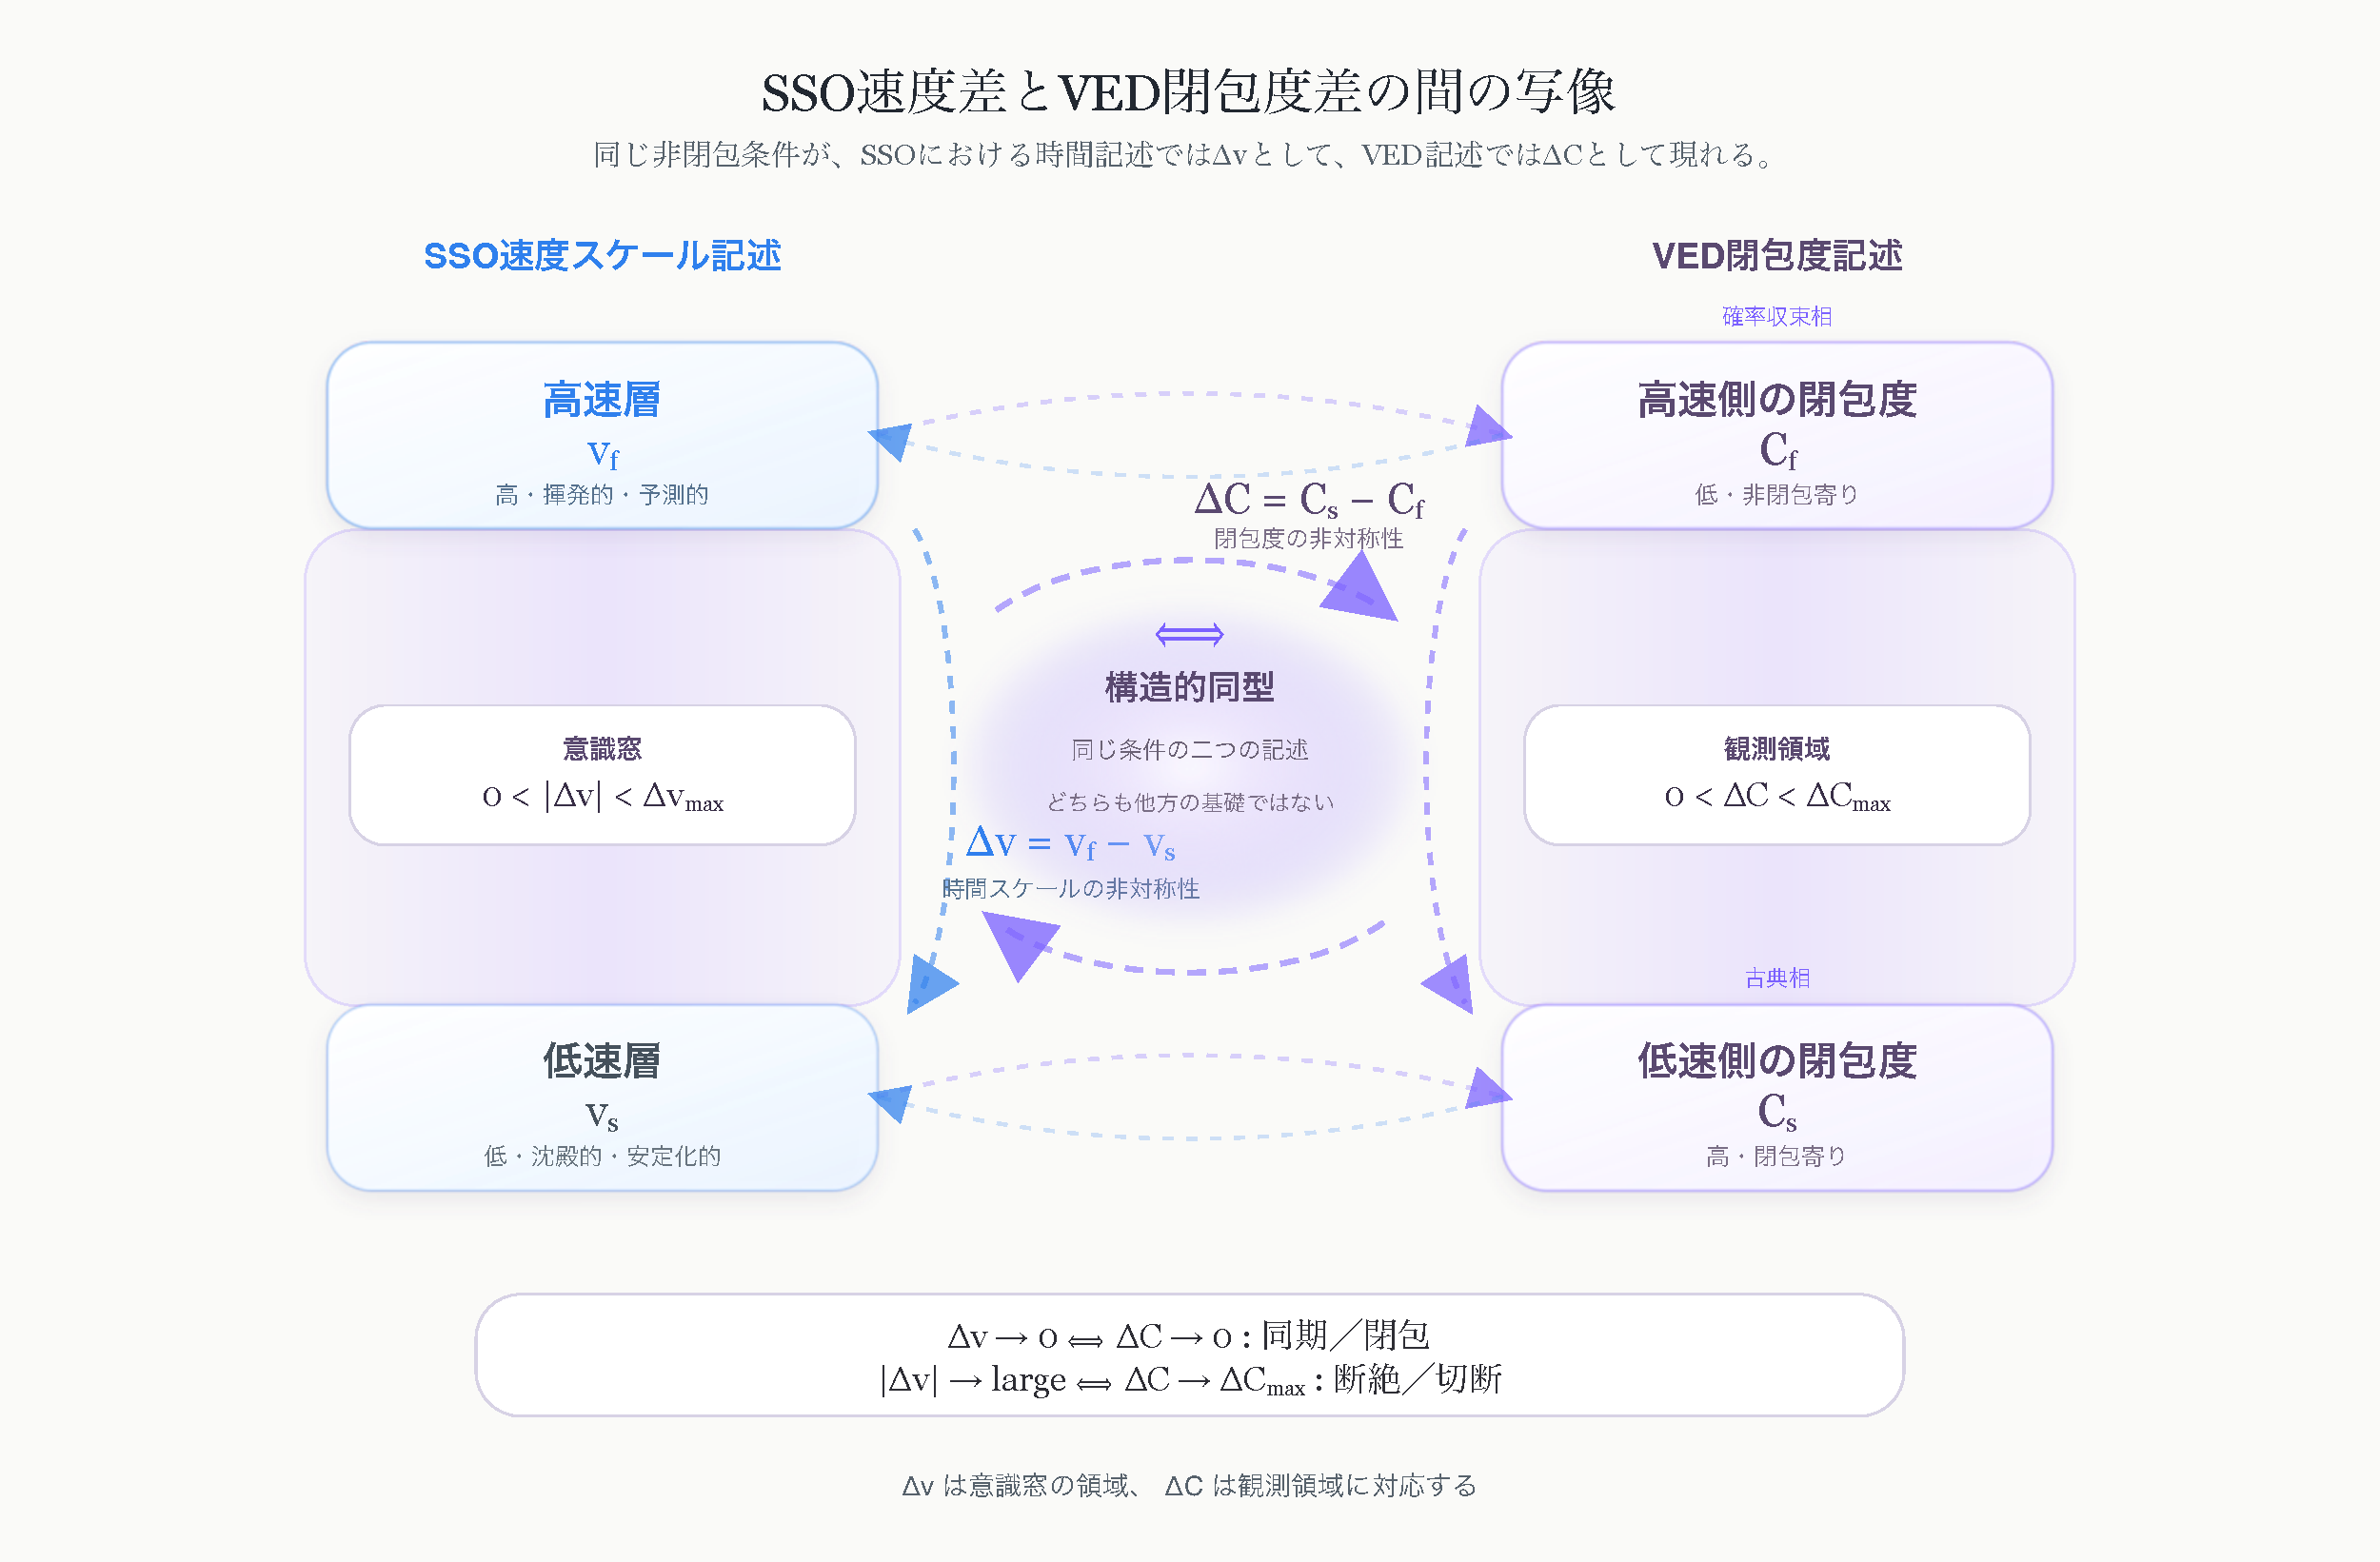
\includegraphics[width=0.94\linewidth]{figures_ja/figure6_observation_regime_jp.pdf}
\caption{
SSO の非対称性と VED の閉包度非対称性の対応。
SSO における速度差 $\Delta v$ と、VED における閉包度差 $\Delta C = C_s - C_f$ は、同じ非閉包条件を異なる座標で記述している。
SSO 側の consciousness window は、VED 側の observation regime に構造的に対応するが、どちらか一方が他方を基礎づけるわけではない。
}
\label{fig:sso-ved-mapping-ja}
\end{figure}

また、旧来の VED における非閉包持続条件

\begin{equation}
\frac{\partial C}{\partial t} + \nabla \cdot J_C = a\Delta\!\left(1 - C/C_*\right) - \Gamma C - \frac{\kappa_B}{C_{\max} - C}
\end{equation}

は、意識モデルにおいて現象論的・粗視化的な近似として次のように読まれる。

第一項 $a\Delta(1 - C/C_*)$ は、差の駆動による閉包への傾向を表す。高速層が低速層を引き寄せようとする力に対応する。

第二項 $-\Gamma C$ は、閉包が進みすぎることへの散逸を表す。完全同期を妨げる項であり、速度差が消滅しないための条件を与える。

第三項 $-\kappa_B/(C_{\max} - C)$ は、閉包が飽和限界に近づくにつれて増大する現象論的な有効障壁を表す。Vol.4 改訂後の解釈では、これは基本的な外部禁止壁ではない。完全閉包が生成された記述の内部で通常状態として実現されないという事実を、射影的な抵抗項として要約したものである。

この三項構造により、SSO は完全閉包にも完全分離にも至らない中間レジームを自己維持的に保つ。

これが、意識状態の非閉包持続条件のVED的根拠である。

\subsection{SSO as Local Non-Closure}

SSO（Speed-Scale Orchestration）は、複数の時間スケールをもつ処理が、中央制御なしに調整される構造である。

VED の観点から見れば、SSO は閉じきらない時間構造の局所モデルである。

高速層は予測し、低速層は沈殿する。

高速層は先に進み、低速層は遅れて固定する。

この差は消されない。

むしろ、この差が残るからこそ、現在処理と過去ログのあいだに参照関係が生まれる。

SSO が成立する条件は、次の三つである。

\begin{enumerate}
\item 高速層と低速層の速度差が存在すること。
\item 両層が完全には分離していないこと。
\item 低速層への沈殿が完全には閉じきっていないこと。
\end{enumerate}

この三条件が満たされるとき、処理は現在に流れ去るだけでなく、過去ログとの関係を開く。

ここに、ログ参照としての意識状態が成立する。

\subsection{Torque Converter Attention as IFGT/VED Coupler}

トルクコンバータ・アテンションは、IFGT と VED の接続点である。

VED 的には、それは速度差 $\Delta v$ を消さずに伝達する非閉包機構である。

IFGT 的には、それは情報ポテンシャル $\Phi$ の勾配に沿って、どのログが参照されやすいかを調整する機構である。

このため、有効トルク様量 $\mathcal{T}$ は、まず速度差と結合粘性によって表される。

\begin{equation}
\mathcal{T} =
\kappa
\frac{\Delta v}{\mu}
\end{equation}

しかし、意識状態において参照されるログは、速度差だけで決まらない。

ログ参照は意味勾配によって方向づけられる。

したがって、意識モデルにおける有効量は、情報ポテンシャルの勾配を含んだ形に拡張される。

\begin{equation}
\mathcal{T}_{\Phi}
\sim
\kappa
\frac{\Delta v}{\mu}
|\nabla \Phi|
\end{equation}

ここで $\mathcal{T}_{\Phi}$ は、時間スケール差と意味勾配が結合した有効トルク様量である。

これは意識を生成する量ではない。

それは、ログ参照がどの程度強く、どの方向へ開かれやすいかを示す構造的指標である。

\subsection{Consciousness as IFGT/VED Interface}

以上を踏まえると、本稿における意識は、IFGT と VED の交差面における局所的な射影レジームとして位置づけられる。

IFGT は、ログ、意味場、情報流の配置を与える。

VED は、その配置が完全閉包を通常状態として実現せず、差と流れを保ち続ける条件を与える。

意識は、この二つの記述が重なるところでモデル化される。

すなわち、意識とは、射影された情報ポテンシャルに方向づけられたログ参照が、完全同期にも完全分離にも至らない時間的非閉包レジームの中で開かれている状態である。

これを最小形で書けば、次のようになる。

\begin{equation}
\text{Consciousness}
\sim
\text{Log Referencing}
\left(
I,
J_{\log},
\Phi,
\Delta v,
\mu,
\tau,
\mathcal{T}_{\Phi}
\right)
\end{equation}

この式は、意識を計算する式ではない。

それは、意識について語るときに必要な構造変数を示す座標である。

意識は、$I$ だけに還元されない。

$J_I$ だけにも、$J_{\log}$ だけにも、$\Phi$ だけにも、$\Delta v$ だけにも還元されない。

意識は、それらが時間的非閉包状態の中で結合したときに開かれる。

\paragraph{差分発展構造の投影としての位置づけ}
本節で固定された IFGT/VED 界面における意識の位置は、より広い構造の中に置かれている。VED は物理層を、Bio-IFGT は生命層を、本稿は意識層を、知性編 \cite{Intelligence} は知性層をそれぞれ記述する。これら四層は同一の差分発展構造を異なる粒度で繰り返しており、各論文はそのうちのひとつの投影窓を記述している。

§\ref{sec:projected-uses-stance} で固定された投影的使用の立場は、この複数窓間の関係を「相互還元」ではなく「同一構造の異なる投影」として読むことを要請する。本稿の意識窓と他層との対応の詳細は §20 で整理される。

\subsection{Why This Mapping Is Minimal}

本節の写像は、意図的に最小限にとどめられている。

理由は二つある。

第一に、意識を過剰に形式化すると、意識を閉じた対象として扱ってしまう危険がある。

しかし本稿の立場では、意識は完全閉包された対象ではなく、非閉包的なログ参照状態である。

第二に、IFGT/VED の役割は、意識を説明しきることではなく、意識についての問いを正しい位置へ置くことである。

したがって、本節では意識の統一方程式を与えない。

与えるのは、意識がどの変数のあいだに開かれるかという、最小対応である。

この最小写像によって、本稿は次節で中核方程式を整理できるようになる。

すなわち、速度差、結合粘性、内部遅延、有効トルク様量、意味勾配、非閉包条件を、同一の構造の中で扱うことが可能になる。
